\chapter{MPMICE: Coupling CFD and MPM} \label{ch:MPMICE}
Approaches to fluid structure interaction (FSI) problems are typically
divided into two classes.  ``Separated" approaches treat individual materials
as occupying distinct regions of space, with interactions occurring only at
material interfaces.  The details of those interactions vary between
implementations, and are often a function of the degree, or ``strength" of the
coupling between the fluid and solid fields.  Because of the separated
nature of the materials, only one set of state variables is needed at any
point in space, since only one material is allowed to exist at that point.
``Averaged" model approaches allow {\bf all} materials to exist at any point in
space with some probability.    Variables describing the material state vary 
continuously throughout the computational domain, thus, the state of every 
material is defined at every point in space.  Distinct material interfaces are 
not defined, rather the interaction between materials is computed in an average 
sense, and, as such, interactions among materials may take place anywhere.

While both the separated model and averaged model approaches have their
respective merits, the averaged model, when carried out on an Eulerian grid,
allows arbitrary distortion of materials and material 
interfaces.  However, these distortions can be catastrophic for the solid 
material, as the deformation history of the solid must be transported through 
the Eulerian grid.  This transport can lead to non-physical stresses and the 
interface between materials is also subject to diffusion.  The latter problem 
can be mitigated via surface tracking and the use of a single valued 
velocity field~\cite{Benson1995,Benson1998}, but this does not eliminate the 
problems of stress transport.

The approach described here uses the averaged model approach, and addresses
the issue of stress transport by integrating the state of the solid field in 
the ``material" frame of reference through use of the Material Point 
Method (MPM)~\cite{Sulsky1994,Sulsky1995}.  MPM is a particle method for 
solid mechanics that allows the solid field to undergo arbitrary 
distortion.  Because the fluid state is integrated in the Eulerian frame, it 
can also undergo arbitrary distortion.  MPM uses a computational ``scratchpad" 
grid to advance the solution to the equations of motion, and by choosing to 
use the same grid used in the Eulerian frame of reference, interactions 
among the materials are facilitated on this common computational 
framework.  By choosing to use an infinitely fast rate of momentum transfer 
between the materials, the single velocity field limit is obtained, and the 
interface between materials is limited to, at most, a few cells.  Thus, in 
the differential limit, the separated model can be recovered.  This means 
that with sufficient grid resolution, the accuracy of the separated model 
and the robustness of the averaged model can be enjoyed simultaneously.

An exposition of the governing equations of the CFD approach are given
in Chapter~\ref{ch:ICETheory} while those for MPM can be found in
Chapter~\ref{ch:MPMTheory}.  Algorithmic description of the solution of those 
equations can also be found in those chapters, but a summary is provided here.
The reader is encouraged to 
browse Section~\ref{sec:numerical_results}  to better appreciate
the direction that the subsequent development is headed.

\section{Numerical Implementation}\label{sec:numerical_algorithm}

A description of the means by which numerical solutions to the equations in 
the preceding section are found is presented next.  This begins with 
separate, brief, overviews of the methodologies used for the Eulerian and 
Lagrangian reference frames.  The algorithmic details necesssary for
integrating them to achieve a tightly coupled fluid-structure interaction 
capability is provided in Sec.~\ref{sec:coupling}.

\subsection{ICE Eulerian Multi-Material Method}\label{sec:EulerianMFM}

The Eulerian method implemented here is a
cell-centered, finite volume, multi-material version of the ICE
(for Implicit, Continuous fluid, Eulerian) method \cite{Harlow1968}
developed by Kashiwa and others at Los Alamos National
Laboratory \cite{Kashiwa1994a}.  ``Cell-centered'' means that all elements
of the state are colocated at the grid cell-center (in contrast to a 
staggered grid,
in which velocity components may be centered at the faces of grid cells, for
example).  This colocation is particularly important in regions where a
material mass is vanishing.  By using the same control volume for mass and
momentum it can be assured that as the material mass goes to zero, the mass
and momentum also go to zero at the same rate, leaving a well defined
velocity.  The technique is fully compressible, allowing wide generality in
the types of problems that can be efficiently computed. 
 
Our use of the cell-centered ICE method employs time splitting: first, a
Lagrangian step updates the state due to the physics of the conservation laws
(i.e., right hand side of Eqs.~{\ref{eq:eqmassr}-\ref{eq:eqenergyr}}); this is
followed by an Eulerian step, in which the change due to advection is
evaluated.  For solution in the Eulerian frame, the method is well developed
and described in \cite{Kashiwa1994a}.  

In the mixed frame approach used here, a modification to the multi-material equation
of state is needed.  Equation~\ref{eq:mmeos} is unambiguous when all materials
are fluids or in cases of a flow consisting of dispersed solid
grains in a carrier fluid.  However in fluid-structure problems the stress
state of a submerged structure may be strongly directional, and the
isotropic part of the stress has nothing to do with the hydrodynamic
(equilibration) pressure $p$.  The equilibrium that typically exists between 
a fluid and a solid is at the interface between the two materials: there the 
normal part of the traction equals the pressure exerted by the fluid on the 
solid over the interface.  Because the orientation of the interface is not 
explicitly known at any point (it is effectively lost in the averaging) such 
an equilibrium cannot be computed.

The difficulty, and the modification that resolves it, can be understood by
considering a solid material in tension coexisting with a gas. 
For solid materials, the equation of state is the bulk part of the
constitutive response (that is, the isotropic part of the Cauchy stress versus
specific volume and temperature).  If one attempts to equate the isotropic
part of the Cauchy stress with the fluid pressure, there exist regions in
pressure-volume space for which Eq.~\ref{eq:mmeos} has no physical solutions
(because the gas pressure is only positive).  This can be seen schematically
in Fig.~\ref{vpfig}, which sketches equations of state for a gas and a 
solid, at an arbitrary temperature.

Recall that the isothermal compressiblity is the negative slope of
the specific volume versus pressure.  Embedded structures considered here are
solids and, at low pressure, possess a much smaller
compressibility than the gasses in which they are submerged.  
Nevertheless the variation of condensed phase specific volume can be important
at very high pressures, where the compressibilities of the gas and condensed
phase materials can become comparable (as in a detonation wave, for
example).  Because the speed of shock waves in materials is determined by
their equations of state, obtaining accurate high pressure behavior is an
important goal of our FSI studies.

To compensate for the lack of directional information for the embedded
surfaces, we evaluate the solid phase equations of state
in two parts.  Above a specified postive threshold pressure 
(typically 1 atmosphere), the full equation of state is respected; below that 
threshold pressure, the solid phase pressure follows a
polynomial chosen to be $C^1$ continuous at the threshold value and
which approaches zero as the specific volume becomes large.  The effect
is to decouple the solid phase specific volume from the stress
when the isotropic part of the stress falls below a threshold value.  In 
regions of coexistence at states below the threshold pressure, $p$ tends 
to behave according to the fluid equation of state (due to the greater 
compressibility) while in regions of pure condensed phase material $p$ tends 
rapidly toward zero and the full material stress dominates the dynamics as 
it should.

\subsection{The Material Point Method}\label{sec:mpm}

Solid materials with history dependent constitutive relations are more 
conveniently treated in the Lagrangian frame.  Here we briefly describe a 
particle method known as the Material Point Method (MPM) which is used to 
evolve the equations of motion for the solid phase materials.  MPM is a 
powerful technique for computational solid mechanics, and has found favor 
in applications involving complex geometries~\cite{Guilkey2006}, large 
deformations ~\cite{Brydon2005} and fracture~\cite{Guo2004}, to name 
a few.  After the description of MPM, its incorporation 
within the multi-material solution is described in 
Sec.~\ref{sec:coupling}.

Originally described by Sulsky, et al., \cite{Sulsky1994,Sulsky1995}, 
MPM is a particle method for structural mechanics simulations.  MPM is an 
extension to solid mechanics of FLIP \cite{brackbill-ruppel86}, which is a 
particle-in-cell (PIC) method for fluid flow simulation.  The method typically
uses a cartesian grid as a computational scratchpad for computing
spatial gradients.  This same grid also functions as an updated Lagrangian grid
that moves with the particles during advection and thus eliminates the
diffusion problems associated with advection on an Eulerian grid.  At the end
of a timestep, the grid is reset to the original, regularly ordered, position.
Details of the theory of \MPM can be found in Chapter~\ref{ch:MPMTheory}.

By describing and implementing MPM in an independent fashion, validation of 
the method itself as well as submodels (e.g., constitutive models and contact)
is simplified.  However, we emphasize that its use here is for selected 
material field description within the general multi-material formulation.  This 
integration is described next.

\subsection{Integration of MPM within the Eulerian Multi-Material 
            Formulation}\label{sec:coupling}

An important feature of this work is the ability to represent a material in 
either the Lagrangian or Eulerian frame.  This allows treating specific phases 
in their traditionally preferred frame of reference.
The Material Point Method, is used to time 
advance solid materials that are best described in a Lagrangian reference frame.
By choosing the background grid used to update the solid materials to
be the same grid used in the multi-material Eulerian description,
all interactions among materials can be computed in the common
framework, according to the momentum and heat exchange terms in 
Eqs~\ref{eq:eqmomr}-\ref{eq:eqenergyr}.  This results in a robust and tightly 
coupled solution for interacting materials with very different responses.

To illustrate how the integration is accomplished in an algorithmic fashion 
the explicit steps for advancing a fluid-structure interaction problem from 
time $t$ to time $t+\Delta{t}$ are described below.
\begin{enumerate}

%\setlength{\topsep=0.1in}
%\setlength{\itemsep=0.0in}
%\setlength{\parskip=0.1in}
%\setlength{\partopsep=0.4in}

\item {\bf Project particle state to grid:} A simulation timestep begins by
interpolating the particle description of the solid to the grid.  This starts
with a projection of particle data to grid vertices, or nodes, as described
in Eq.~\ref{accumulate}, and is followed by a subsequent projection from
the nodes to the cell-centers.  Since our work uses a uniform structured
grid, each node has equal weight in its contribution to the cell-centered
value.  The exception to this is near computational boundaries where
symmetric boundary conditions are used.  The weight of those nodes on
the boundary must be doubled in order to achieve the desired effect.

\item {\bf Compute the equilibrium pressure:} While Eq.~\ref{eq:mmeos} and the
surrounding discussion describes the basic process, one specific point warrants
further explanation.  In particular, the manner in which each material's
volume fraction is computed is crucial.  Because the solid and fluid materials 
are evolved in different frames of reference, the total volume of material in a 
cell is not necessarily equal to the volume of a computational cell.  Material 
volume is tracked by evolving the specific volume for each material 
according to Eq.~\ref{eq:eqspvolr}.
The details of this are further described in step 11.

With the materials' masses and specific volumes, material volume
can be computed ($V_r=M_r v_r$) and summed to find the total material volume.  The volume
fraction $\theta_r$ is then computed as the volume of r-material per total
material volume.  With this, the solution of Eq.~\ref{eq:mmeos} can be carried
out at each cell using a Newton-Raphson technique\cite{Harlow1975},
which results in new values for the equilibrium pressure, $p_{\Teq}$,
volume fraction, $\theta_r$ and specific volume, $v_r$.

\item {\bf Compute face-centered velocities, $u^*_r$, for the 
           Eulerian advection:}
At this point, fluxing velocities are computed at each cell face.  The 
expression for this is based on a time advanced estimate for the cell-centered 
velocity.  A full development can be found in  \cite{Kashiwa1994a} and 
\cite{Kashiwa2000} but here, only the result is given:
\begin{equation}
u^*_r = \frac{\rho_{r_L} u_{r_L} + \rho_{r_R} u_{r_R}}
                {\rho_{r_L} + \rho_{r_R}} -
           \left( \frac{2 v_{r_L} v_{r_R} \Delta{t}}
                       {v_{r_L} + v_{r_R}}\right)
           \left( \frac{p_{{\Teq}_R} - p_{{\Teq}_L}}{\Delta{x}}\right) + g\Delta{t}
\end{equation}
The first term above is a mass weighted average of the logically left and right
cell-centered velocities, the second is a pressure gradient acceleration
term, and the third is acceleration due to the component of gravity in the face 
normal direction.  Not shown explicitly is the necessary momentum exchange at the
face-centers.  This is done on the faces in the same manner as described subsequently
in step 10 for the cell-centered momentum exchange.

\item {\bf Multiphase chemistry:} Compute sources of mass, momentum, energy
and specific volume as a result of phase changing chemical reactions for 
each r-material, $\Gamma_r$, $u_r \Gamma_r$, $e_r \Gamma_r$,
and $v_r \Gamma_r$.  Specifics of the calculation of $\Gamma_r$ are 
model dependent, and examples are given in Sec.~\ref{sec:HEReaction}.

Care must be taken to reduce the momentum, internal energy and volume of the 
reactant by an amount proportional to the mass consumed each timestep, so that 
those quantities are depleted at the same rate as the mass.  When the reactant 
material is described by particles, decrementing
the particle mass automatically decreases the momentum and internal energy
of that particle by the appropriate amount. This mass, momentum, 
and internal energy is transferred to the product material's state, 
and the volume fraction for the reactant and product materials is recomputed.

\item {\bf Compute an estimate of the time advanced pressure, $p$:}  Based on
the volume of material being added to (or subtracted from) a cell in a given 
timestep, an increment to the cell-centered pressure is computed using:

\begin{eqnarray}
     \Delta p &=&
     \DelT~ \frac{ \sum\limits_{r=1}^N v_r\Gamma_r
    -\sum\limits_{r=1}^N \nabla \cdot (\theta^{*}_r {u}^{*}_r)}
     {\sum\limits_{r=1}^N \theta_r\kappa_r}
    \label{eq:delP} \\
    p&=&p_{\Teq}+\Delta p \label{eq:time_adv_press}
\end{eqnarray}
where $\kappa_r$ is the r-material bulk compressibility.  The first term in 
the numerator of Eq.~\ref{eq:delP} represents the change in volume due to 
reaction, i.e., a given amount of mass would tend to occupy more volume in 
the gas phase than the solid phase, leading to an increase in pressure.  The 
second term in the numerator represents the net change in volume of material 
in a cell due to flow into or out of the cell.  The denominator is essentially 
the mean compressibility of the mixture of materials within that cell.  
This increment in pressure 
is added to the equilibrium pressure computed in step 2 and is the pressure 
used for the remainder of the current timestep.  Again, the details leading
to this equation can be found in \cite{Kashiwa1994a}.

\item {\bf Face Centered Pressure $p^*$:}
The calculation of $p^*$ is discussed at length in \cite{Kashiwa2000}.
For this work, it is computed using the updated pressure by:
\begin{equation}
p^* = {\left (\frac{p_L}{\rho_L} + \frac{ p_R}{\rho_R}\right)}/
                     {\left (\frac{1}{\rho_L} + \frac{1}{\rho_R}\right)}
\end{equation}
where the subscripts $L$ and $R$ refer to the logically left and right 
cell-centered values, respectively, and $\rho$ is the sum of all material's 
densities in that cell.  This will be used subsequently for the computation 
of the pressure gradient, $\nabla{ p^*}$.

\item {\bf Material Stresses:} For the solid, we calculate the velocity
gradient at each particle based on the grid velocity (Eq.~\ref{velgrad}) for use
in a constitutive model to compute particle stress.  Fluid stresses are
computed on cell faces based on cell-centered velocities.

\item {\bf Accumulate sources of mass, momentum and energy at cell-centers:}
These terms are of the form:
\begin{eqnarray}
%mass
 \Delta(m)_r &=& \DelT~ V \sum\limits_{s=1, s\ne r}^N \Gamma_s 
   \label{deltamass}\\
 %momentum
 \Delta(mu)_r &=& -\DelT~ V \left[\theta_r\nabla{ p^*} 
 + \nabla{ \cdot \theta_r (\Bsig_r - \Bsig) }
 + \sum_{s=1, s\ne r}^N u_s \Gamma_s\right] \label{deltamom} \\
 %energy
 \Delta(me)_r &=&  -\DelT~ V \left[\fthetar p
     \sum\limits_{s=1}^N \nabla \cdot (\theta^{*}_r {u}^{*}_r)
 + \sum\limits_{s=1, s\ne r}^N e_s \Gamma_s \right] \label{deltenergy}
 \end{eqnarray}
Note that the only source of internal energy
being considered here is that due to ``flow work".  This is required 
for the compressible flow formulation, but other terms, such as heat 
conduction are at times included.

\item {\bf Compute Lagrangian phase quantities at cell-centers:} The
increments in mass, momentum and energy computed above are added
to their time $t$ counterparts to get the Lagrangian values for these 
quantities.
Note that here, some Lagrangian quantities are denoted by an $L-$ superscript.
This indicates that all physical processes have been accounted for except for
inter-material exchange of momentum and heat which is described in the following step.

 \begin{eqnarray}
 (m)_r^L &=& (m)_r^t + \Delta(m)_r \label{lagmass} \\
 (m u)_r^{L-} &=& (mu)_r^t + \Delta(mu)_r \label{lagmom} \\
 (m e)_r^{L-} &=& (m e)_r^t + \Delta(m e)_r \label{lagenergy}
\end{eqnarray}

\item {\bf Momentum and heat exchange:} The exchange of momentum and heat 
between materials is computed according to:
\begin{eqnarray}
(m u)_r^L &=& (m u)_r^{L-} +
  \DelT~ m_r 
  \sum\limits_{s=1}^N \theta_r\theta_s K_{rs}(u_s^L - u_r^L) 
  \label{eqmomex} \\
(m e)_r^L &=& (m e)_r^{L-}+ 
  \DelT~m_r~ c_{v_r} 
  \sum\limits_{s=1}^N \theta_r 
     \theta_s H_{rs}\left(T_s^L - T_r^L \right) \label{eqheatex}
\end{eqnarray}
These equations are solved in a pointwise implicit manner that allows 
arbitrarily large momentum transfer to take place between materials.  Typically,
in FSI solutions, very large ($10^{15}$) values of $K$ are used, which results
in driving contacting materials to the same velocity.  Intermaterial heat
exchange is usually modeled at a lower rate.  Again, note that the same 
operation must be done following Step 3 above in the computation of the 
face-centered velocities.

\item {\bf Specific volume evolution:} As discussed above in step 2, in order to
correctly compute the equilibrium pressure and the volume fraction, it is necessary
to keep an accurate accounting of the specific volume for each material.  Here, 
we compute the evolution in specific volume due to the changes in temperature 
and pressure, as well as phase change, during the foregoing Lagrangian 
portion of the calculation, according to:
\begin{eqnarray}
  \Delta(mv)_r &=& \DelT~ V 
     \left[ v_r \Gamma_r 
        + \fthetar \nabla \cdot \sum\limits_{s=1}^N{\theta_s^*u_s^*}
               + \theta_r \beta_r \dot{T_r} 
        - \fthetar \sum\limits_{s=1}^N{\theta_s \beta_s \dot{T_s}}\right]   
     \label{eq:eqspvoldiscrete} \\
  (mv)_r^L &=& (mv)_r^n + \Delta(mv)_r \label{eq:eqspvolLag}
\end{eqnarray}
where $\beta$ is the constant pressure thermal expansivity and
$\dot{T}=\frac{T^L - T^t}{\Delta{t}}$ is the rate of change of each material's
temperature during the Lagrangian phase of the computation.

\item {\bf Advect Fluids:} For the fluid phase, use a suitable advection scheme,
such as that described in \cite{Kashiwa1998}, to transport mass, momentum, internal energy 
and specific volume.  As this last item is an intensive quantity, it is converted
to material volume for advection, and then reconstituted as specific volume
for use in the subsequent timestep's equilibrium pressure calculation.

\item{\bf Update Nodal Quantities for Solid Materials:}  Those changes in 
solid material mass, momentum and internal energy that are computed at the 
cell-centers are interpolated to the nodes as field quantities, e.g., changes 
in momentum are expressed as accelerations, for use in Eq.~\ref{MPM:euler}.

\item {\bf Advect Solids:} For the solid phase, interpolate the time advanced
grid velocity and the corresponding velocity increment (acceleration) back 
to the particles, and use these to advance the particle's position and 
velocity, according to Eqs.~\ref{MPM:updateVpXp}.

\end{enumerate}

This completes one timestep.  In the preceding, the user has a number of
options in the implementation.  The approach taken here was to develop a 
working MPM code and a separate working multi-material ICE code.  In 
addition, some routines specific to the integration are required, for 
example, to transfer data from grid nodes to cell-centers.  We 
note, however, that the fluid structure interaction methodology should 
not be looked at in the context of a ``marriage" between an Eulerian CFD 
code and MPM.  The underlying theory is a multi-material description
that has the flexibility to incorporate different numerical descriptions for 
solid and fluid fields within the overarching solution process. 
To have flexibility in treating a widest range of problems, it was our 
desire that in the integration of the two algorithms, each of the components 
be able to function independently.  As described here, this method is fully 
explicit in time.  To make this implicit with respect to the propagation 
of pressure waves, a Poisson equation is solved in the calculation of 
$\Delta p$, which is in turn used to iteratively update the face-centered 
velocities \cite{Kashiwa1994a}.

\section{Models}\label{sec:models}

The governing equations given in Section~\ref{sec:governing_equations} are 
incomplete without closure equations for quantities such as pressure, stress, 
and rate of exchange of mass between materials.  Equations of 
state, constitutive models and reaction models provide
the needed closure.  Some ICE material models have been discussed in
Chapter~\ref{ch:ICEMaterials}.  Materials used by the \MPM component are
discussed elsewhere in the Vaango Theory Manual.

\section{Numerical Results}\label{sec:numerical_results}

  The simulation results presented here are intended to serve two purposes, to 
  validate the method presented above, and to demonstrate its 
  capabilities.  While results from some very basic validation tests can be 
  found in \cite{fourthmit}, the validation tests presented here are 
  targeted toward exploding energetic devices.  Extensive experimental data have
  been collected for the first two cases, and these data are compared with 
  simulation results.  
  
  The first test, detonation of a series of cylinders of explosive, validates 
  both the general multi-material framework, including material 
  transformation, as well as the detonation model itself.  In the second 
  test, a cylinder of explosive confined in a copper tube is 
  detonated.  There, the confidence gained from the 
  first test is built upon and extended to include the interaction of the highly
  pressurized product gases with the confining copper cylinder.  Wall velocity 
  of the copper tube is compared with experimental measurements.

  For the last case, a steel cylinder filled with PBX-9501 is heated to the 
  critical temperature to commence a deflagration.  The simulation continues 
  through the rupture of the case when product gases are 
  free to interact with the surrounding air.  This simulation demonstrates a 
  unique capability of this approach, in which initially separate fluid 
  regions are allowed to interact following the failure of the steel container.

\subsection{Rate Stick Simulations}

A well known phenomenon of detonating solid high explosives is the 
so-called ``size effect".  The size effect refers to the change of the 
steady state detonation velocity of explosives, $U_s$ with size $R_0$
\cite{JWLpp}.  In order to validate our implementation of the JWL++ 
detonation model within our multi-material framework, a parameter study 
was conducted for cylinders of Ammonium Nitrate Fuel Oil (ANFO-K1) with 
length of 10 cm and radii ranging from 4 mm to 20 mm.  In addition, a 
one-dimensional simulation provided for the ``infinite radius" case.  In each of the finite radius 
cases, the cylinder was initially surrounded by air.  Detonation was 
initiated by impacting the cylinder at 90 m/s against the boundary of the 
computational domain, at which a zero velocity Dirichlet boundary condition 
was imposed.  This impact was sufficient to raise the pressure within the 
cylinder to above the threshold for initiation of reaction.  The detonation 
velocity was determined by comparing the arrival time of the detonation at 
two points along the cylinder, sufficiently into the far field that the
detonation had reached a steady state.

Material properties for these cases included the following:  The reactant was 
described by a Murnaghan equation of state with parameters $n$ = 7.4, 
$\kappa$ = 3.9$\times$10$^{11}$ Pa$^-1$ and $\rho_0$ = 1160.0 kg/m$^3$.  The products of 
reaction were described by a JWL C-term form  equation of state with parameters
$A$ = 2.9867$\times$10$^{11}$ Pa, $B$ = 4.11706$\times$10$^9$ Pa, $C$ = 7.206147$\times$10$^8$ Pa, $R_1$ = 4.95, 
$R_2$ = 1.15, $\omega$ = 0.35 and $\rho_0$ = 1160.0 kg/m$^3$.  The JWL++ parameters 
were taken as: $G$ = 3.5083$\times$10$^{-7}$ s$^{-1}$Pa$^b$, $b$ = 1.3, $\rho_0$ = 1160.0 kg/m$^3$.  
In all, this simulation included 3 materials; the reactant material, the 
products of reaction and the surrounding air.

Simulations were carried out on uniform meshes with cell sizes of 1.0 mm, 
0.5 mm and 0.25 mm.  A one-quarter symmetry was assumed in all cases.  A 
qualitative representation is shown in Figure \ref{figRSVR}, which depicts a 
volume rendering of the density of the reactant as the detonation has progressed
about halfway into the material for the 12 mm radius case at the finest 
resolution.  The curvature of the burn front and the elevated density just 
ahead of it are evident in this view.

\begin{figure}
  \center
  \scalebox{0.5}{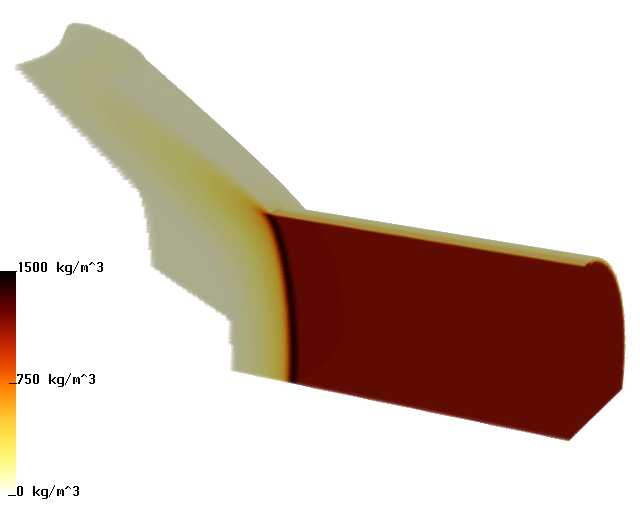
\includegraphics{Figs/mpmice/12mmRSVolRen.png}}
  \caption{Unconfined 12 mm ``rate-stick".  The mass density of the reactant 
           material is volume rendered, and shows evidence of the curvature 
           of the reaction front, and the compression of the reactant just 
           ahead of the reaction.  Behind the detonation, most of the reactant 
           material is consumed. }
  \label{figRSVR}
\end{figure}

Figure \ref{figRSSE} is  a plot of detonation velocity {\it{versus}} the inverse of 
the sample radius.  Experimental data are represented by open squares, 
while results of the simulations are shown with filled circles (h = 1.0 mm), filled
diamonds (h = 0.5 mm) and filled triangles (h = 0.25 mm).  Connecting lines for 
the numerical data are in place to guide the eyes of the reader.  Evident 
from this plot is the convergence of detonation velocities with grid 
resolution, and the generally good agreement between experimental and
computed detonation velocities at the finer grid resolutions, particularly 
at the larger radii, where both the experimental data and the model are 
considered more reliable.

\begin{figure}
  \center
  \scalebox{0.5}{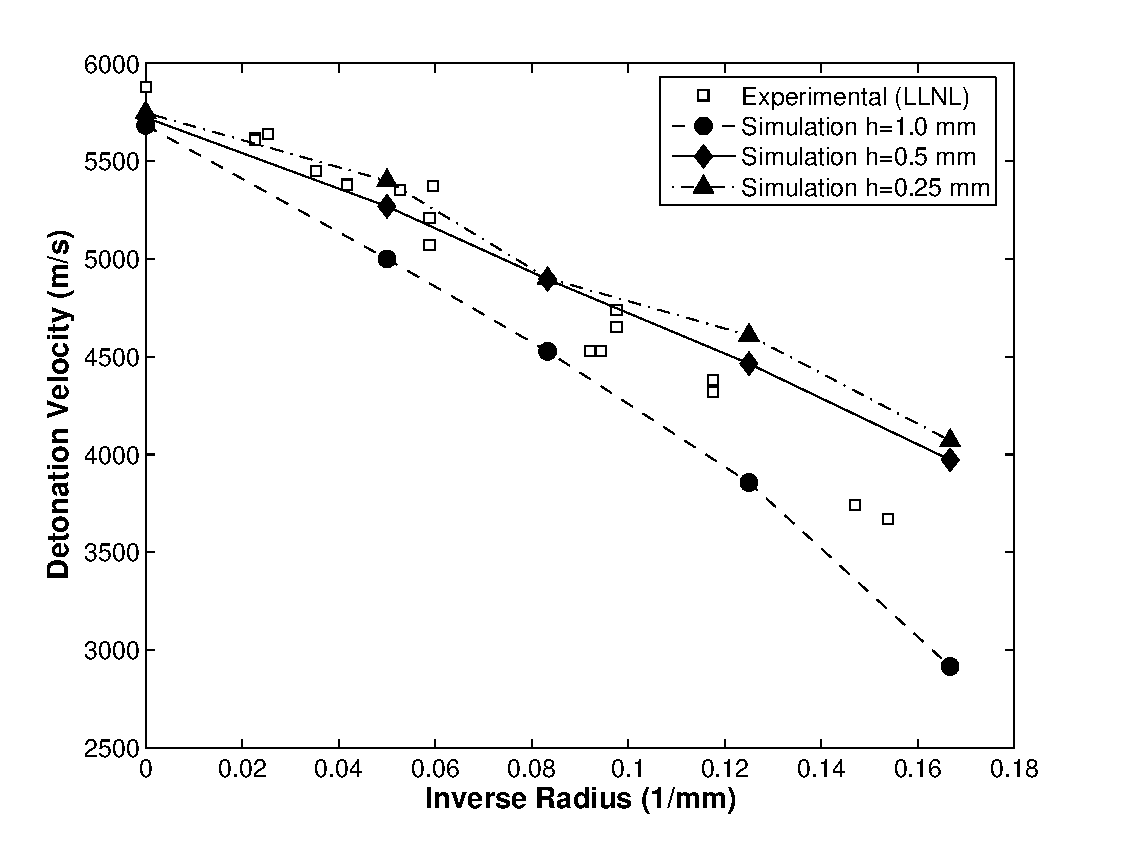
\includegraphics{Figs/mpmice/RateStick.pdf}}
  \caption{Detonation velocity vs. inverse radius.  Experimental and numerical 
          data are presented, and indicate good agreement of the model 
          with experiment, as well as convergence of detonation velocity 
          with grid resolution.}
  \label{figRSSE}
\end{figure}

Again, while this set of tests doesn't validate the full fluid-structure 
interaction approach, it does give credibility to the underlying 
multi-material formulation, including the pressure equilibration and the
exchange of mass between materials, in this case as governed by the 
JWL++ detonation model, as well as momentum and energy.

\subsection{Cylinder Test Simulation}

The cylinder test is an experiment which is frequently used to calibrate 
equations of state for detonation products of 
reaction~\cite{Souers2001CylinderTest}.  In this case, the test consists of an OFHC
copper tube with an inner radius of 2.54 cm, an outer radius of 3.06 cm and 
a length of 35 cm.  The tube is filled with QM-100, an Ammonium Nitrate 
emulsion and a detonation is initiated at one end of the tube.  Measurements
of the wall velocity wall are made at individual points along the length of 
the tube using Fabry-Perot interferometry or streak cameras.

A simulation of this configuration was performed and wall velocity data were 
collected at an axial location 25 cm from the point of initiation.  The 
reactant was again described by a Murnaghan equation of state with parameters 
$n$ = 7.0, $\kappa$ = 1.02$\times$10$^{-9}$ Pa$^{-1}$ and $\rho_0$ = 1260.0 kg/m$^3$.  The products 
of reaction were described by a JWL C-term form  equation of state with 
parameters $A$ = 4.8702$\times$10$^{11}$ Pa, $B$ = 2.54887$\times$10$^9$ Pa, $C$ = 5.06568$\times$10$^8$ Pa, 
$R_1$ = 5.0, $R_2$ = 1.0, $\omega$ = 0.3 and $\rho_0$ = 1260.0 kg/m$^3$.
The JWL++ parameters were taken as: $G$ = 9.1$\times$10$^{-5}$s$^{-1}$ Pa, $b$ = 1.0,
$\rho_0$ = 1260.0 kg/m$^3$.  The copper tube was modeled as an elastic-perfectly 
plastic material with a density of 8930.0 kg/m$^3$, bulk and shear moduli of 
117.0 GPa and 43.8 GPa, respectively,and a yield stress of 70.0 MPa.
The copper tube was surrounded by air.  In all, 4 materials are present in
this simulation, the reactant, the products of reaction, the copper tube, and 
the surrounding air.

Again, a one-quarter symmetry section of the full cylinder was modeled using 
a cell size of h = 0.5 mm and a total domain size of 
35 cm $\times$ 6 cm $\times$ 6 cm.  Zero gradient conditions described the 
exterior boundaries, which allowed material to exit the domain.

Figure \ref{figCuRSiso} shows a snapshot of this test midway through the 
simulation, at t = 18.8 $\mu$s.  The copper tube is depicted using an 
iso-surface of the cell-centered mass density (the two surfaces are the 
inner and outer walls of the tube) that is colored by velocity.  A volume 
rendering of the pressure field is also present.  Alternating bands of high 
and low velocity of the tube wall are evidently due to the reflection of the 
impulse provided by the shock between the inner and outer surfaces of the tube.

\begin{figure}
  \center
  \scalebox{0.5}{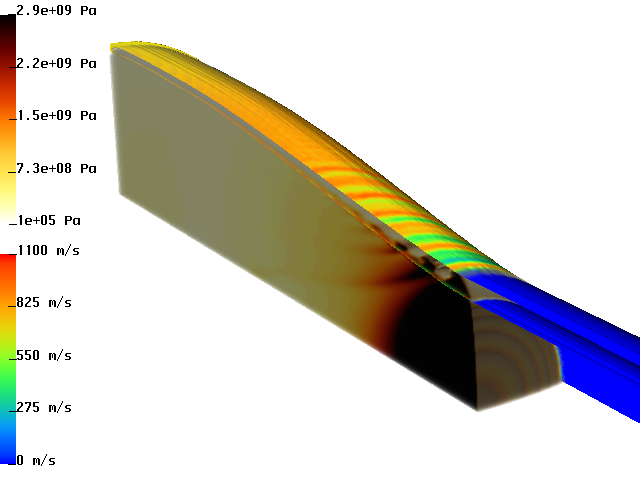
\includegraphics{Figs/mpmice/CuRS1.png}}
  \caption{Copper cylinder test simulation.  The walls of the copper tube 
           are depicted as an isosurface of density of the copper material 
           and are colored by velocity magnitude.  Pressure is represented by a
           volume rendering, and indicates the progress of the detonation, as 
           well as the interaction of the pressurized products of reaction 
           with the confining walls. }
  \label{figCuRSiso}
\end{figure}

Velocity data was collected from those particles which were both initially 
at an axial location of 25 cm, and upon the exterior surface of the tube.  The 
velocity from this collection of particles was averaged over the circumference 
and plotted vs. time in Figure \ref{figCuRSwallvel}.  In addition, experimental 
results (LLNL, Shot No. K260-581) are also shown.  Both datasets are time 
shifted to coincide with the arrival of the detonation.  Good agreement is 
evident between the experimental and numerical data, further indicating the 
validity of the approach described here.

\begin{figure}
  \center
  \scalebox{0.5}{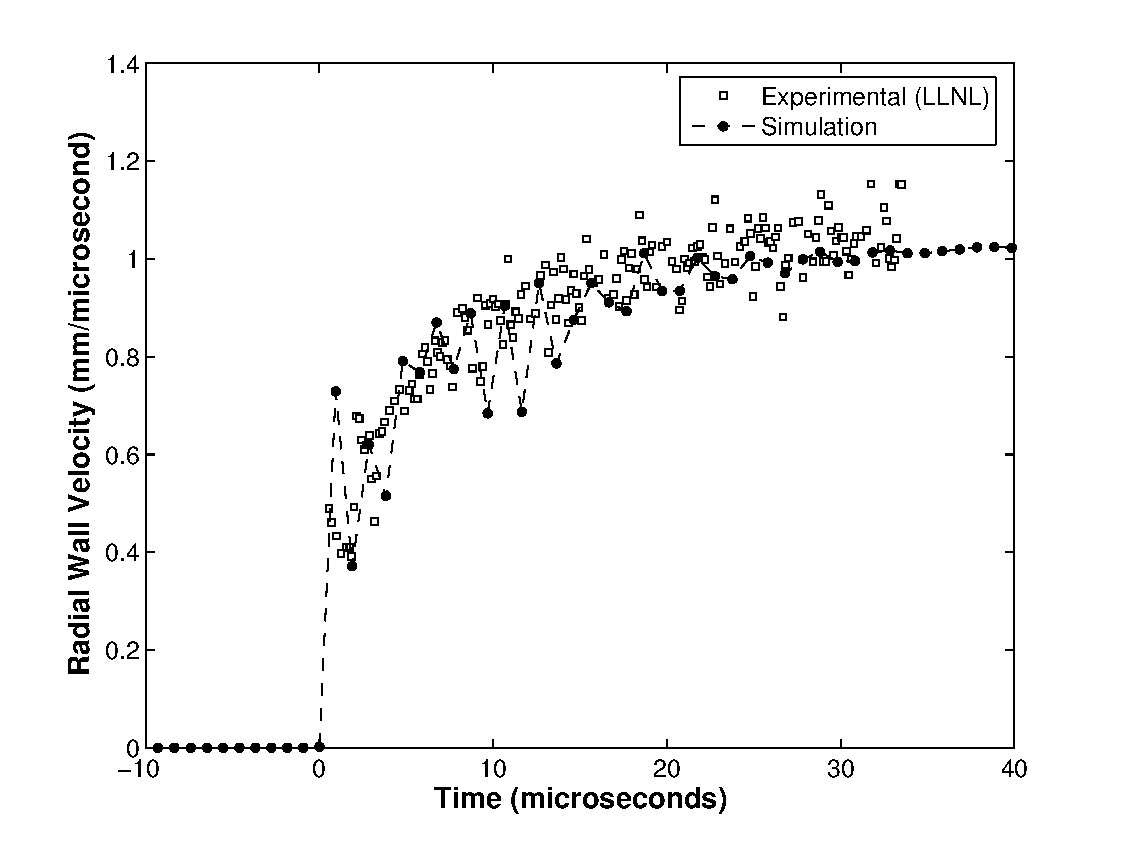
\includegraphics{Figs/mpmice/CuTubeWallVel.pdf}}
  \caption{Copper cylinder test simulation.  Experimental and computational 
           velocities of the cylinder vs. time. Data was collected at a 
           point 25 cm from the point of initiation of the detonation. }
  \label{figCuRSwallvel}
\end{figure}

\subsection{Fast Cookoff Simulation}

Cookoff tests, generally speaking, refer to experiments in which
energetic material is heated until it reaches ignition.  The rate of
heating typically differentiates these tests in to ``fast" or ``slow"
cookoff.  In slow cookoff tests, the temperature is usually increased
very slowly, perhaps a few degrees per hour, so that the entire sample is able to
equilibrate and is nearly isothermal when ignition occurs.  In fast
cookoff tests, heat is added to the system quickly, which is likely
to lead to relatively local ignition at the surface of the sample.  Fast
cookoff is more likely to occur in an accident scenario, where ordinance
may be subject to heating by a fire, as occurred on the USS Forrestal
in 1967.

The scenario considered here consists of a cylindrical 4340 steel container
with both inner diameter and length of 10.16 cm, and wall thickness of
0.635 cm, filled with PBX-9501.  The temperature of the container
was initialized to be 1$^o$ K above the ignition temperature in the
deflagration model for PBX-9501.  In this way, 
the entire outer surface
of the explosive is ignited simultaneously.  This is, of course, somewhat
unrealistic for an accident scenario, but rather is an idealization.

  Mechanical properties for PBX 9501 were obtained from the
  literature~\cite{Hackett2000Viscoscram}, while
  the material constants used in the modeling of 4340 steel are shown in
  Table~\ref{tab:matConst4340}.  A temperature-dependent specific heat model
  \cite{Goto2000} was used to compute the internal energy and the rate of 
  temperature increase in the material.  We assumed an initial mean porosity 
  of 0.005 with a standard deviation of 0.001.  The critical porosity was 0.3.
  The mean strain at void nucleation was assumed to be 0.3 with a standard 
  deviation of 0.1.  The scalar damage variable was initialized with a mean
  of 0.005 and a standard deviation of 0.001.
  
    \begin{table}[t]
    \caption{Material constants for 4340 steel.}
    \label{tab:matConst4340}
    \centering
    \small
    \renewcommand{\arraystretch}{1.25}
    {
    \begin{tabular}{cccccccccc}
    \hline\hline
    $\rho$    & $K$   & $\mu$ & $T_0$ & $T_m$ &$C_0$&$\Gamma_0$&$S_{\alpha}$ \\
    (kg/m$^3$)& (GPa) & (GPa) & (K)   & (K)   &(m/s)&          &             \\
    \hline
    7830.0    & 173.3 & 80.0  & 294.0 & 1793.0& 3574  & 1.69 & 1.92 \\
    \hline
    \hline
    $A$   & $B$   & $C$   & $n$  & $m$  & $D_1$ & $D_2$ & $D_3$ & $D_4$ &$D_5$\\
    (MPa) & (MPa) &       &      &      &       &       &       &       & \\
    \hline
    792.0 & 510.0 & 0.014 & 0.26 & 1.03 & 0.05  & 3.44  & -2.12 & 0.002 & 0.61\\
    \hline
    \end{tabular}
    }
  \end{table}

Three planes of symmetry are assumed, which allows modeling only 1/8th
of the total geometry.  Each dimension of the computational domain
was 9.0 cm discretized into 180 computational cells,
for a grid spacing of h = 0.5 mm.  Four materials were present,
the steel container and the PBX-9501, each of which are treated in
the Lagrangian frame of reference, as well as the air initially surrounding
the container, and the products of reaction from the deflagration, both
of which are represented in the Eulerian frame of reference.  Neumann
zero gradient boundary conditions are used on the exterior domain
boundaries to allow material to flow out of the domain, as the explosion
progressed.

Because of the size and complexity of this simulation, significant
computational resources were required to obtain a solution.  Namely,
the simulation ran for about 48 hours on 600 processors of a Linux
cluster at Lawrence Livermore National Laboratory, which resulted in
0.31 milliseconds of simulated time.

Results from this simulation are shown in Fig.~\ref{figCookoff}.  In
each panel, the container and explosive are depicted by isosurfaces,
blue and red, respectively.  In Fig.~\ref{figCookoff:b}-\ref{figCookoff:e},
a volume rendering of the mass density of the product material of the
reaction is also included.  Fig.~\ref{figCookoff:a} shows the initial
state of the geometry, while the remaining panels show the progression
of the simulation at the times indicated in the captions.  The last
two panels depict the same time, with the product gas removed in the
final panel, to more clearly show the state of the container at that
time.  Close comparison of the initial and final panels also reveals
the reduction in size of the explosive pellet, due to the reaction.
Product gas first begins to leave the container through a
rupture where the side and end of the container
meet(Fig.~\ref{figCookoff:c}), and ultimately
also through a rupture in middle (Fig.~\ref{figCookoff:e}).  The
formation of these openings is governed by material localization.
\begin{figure}[t!]
 \centering
 \begin{subfigure}[b]{0.3\textwidth}
   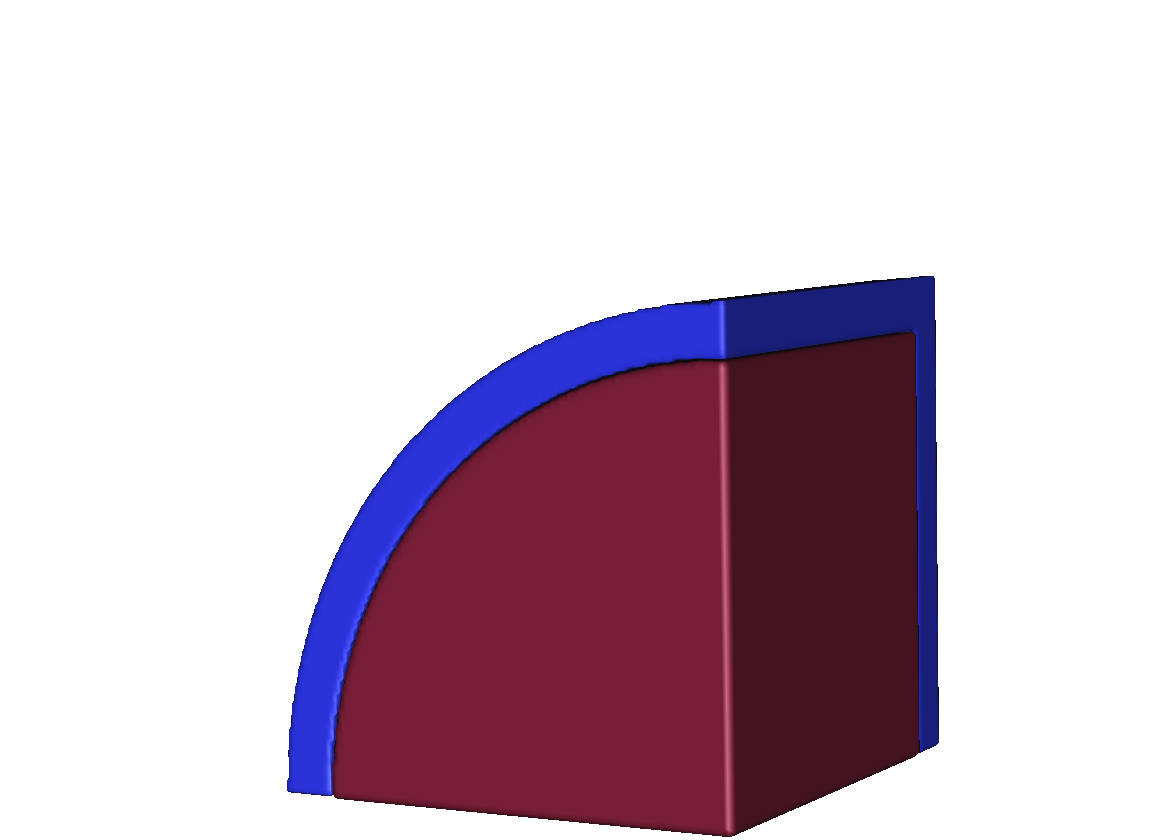
\includegraphics[width=\textwidth]{Figs/mpmice/NE_0_d.png}
   \caption{t=0 $ms$}
   \label{figCookoff:a}
 \end{subfigure}
 \begin{subfigure}[b]{0.3\textwidth}
   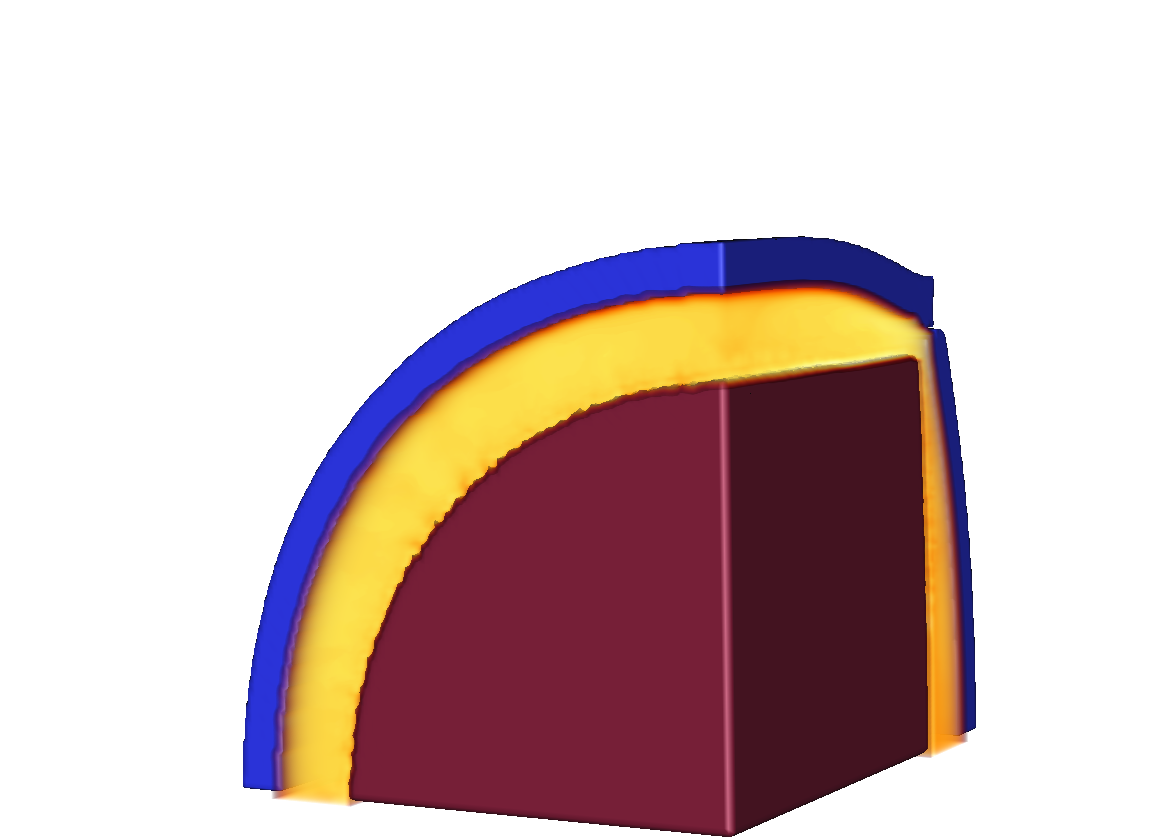
\includegraphics[width=\textwidth]{Figs/mpmice/NE_46_c.png}
   \caption{t=.137 $ms$}
   \label{figCookoff:b}
 \end{subfigure}
 \begin{subfigure}[b]{0.3\textwidth}
   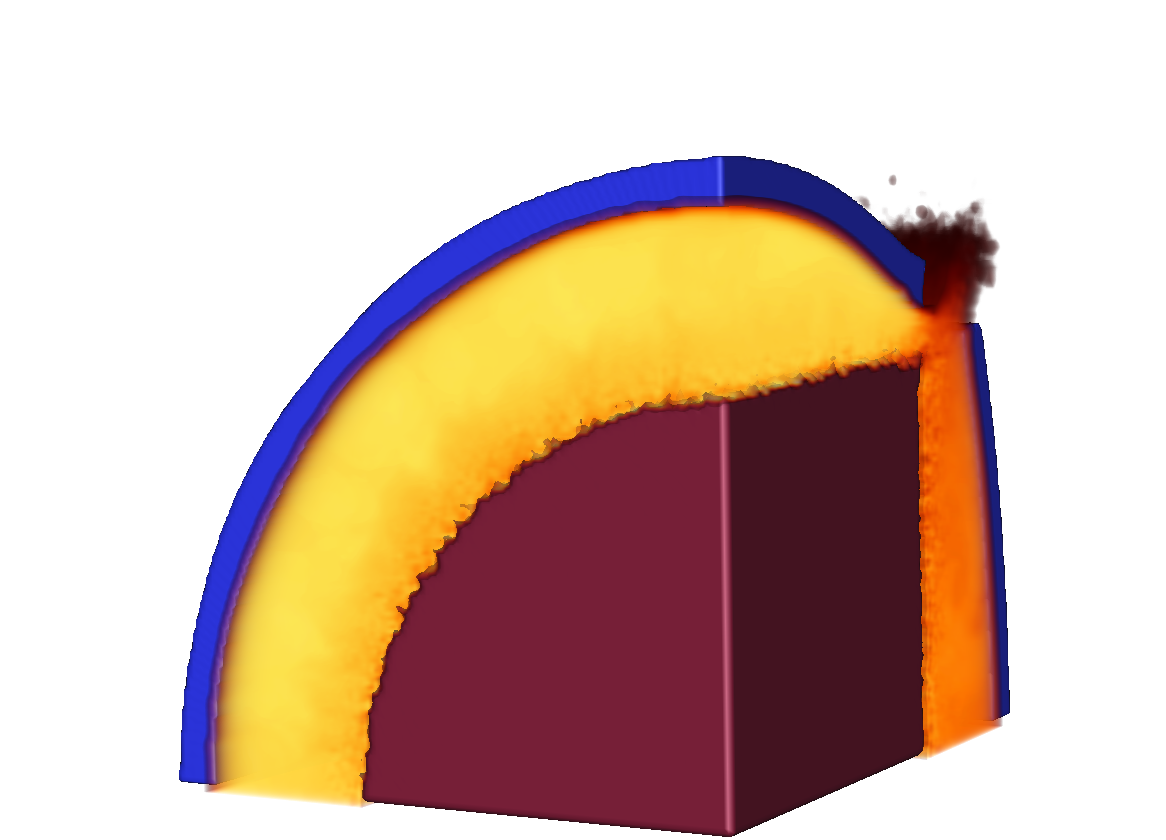
\includegraphics[width=\textwidth]{Figs/mpmice/NE_98_c.png}
   \caption{t=.203 $ms$}
   \label{figCookoff:c}
 \end{subfigure}
 \begin{subfigure}[b]{0.3\textwidth}
   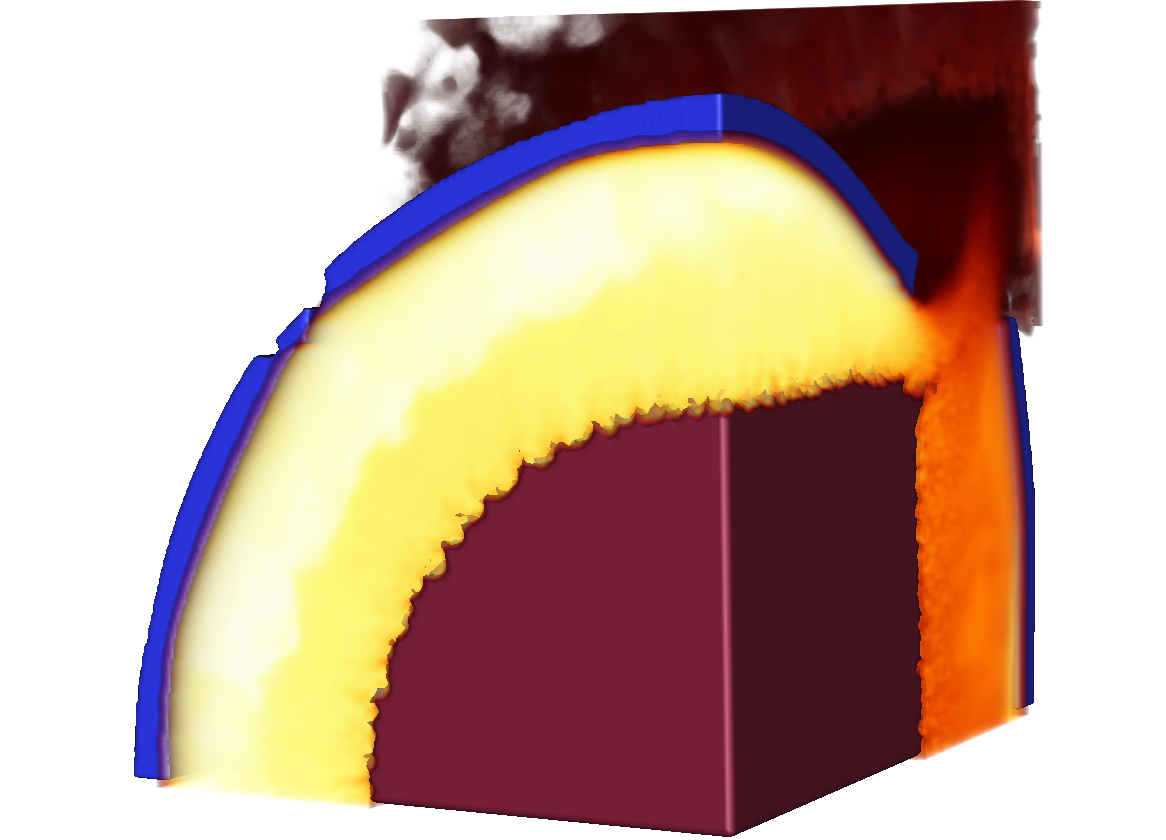
\includegraphics[width=\textwidth]{Figs/mpmice/NE_129_c.png}
   \caption{t=.259 $ms$}
   \label{figCookoff:d}
 \end{subfigure}
 \begin{subfigure}[b]{0.3\textwidth}
   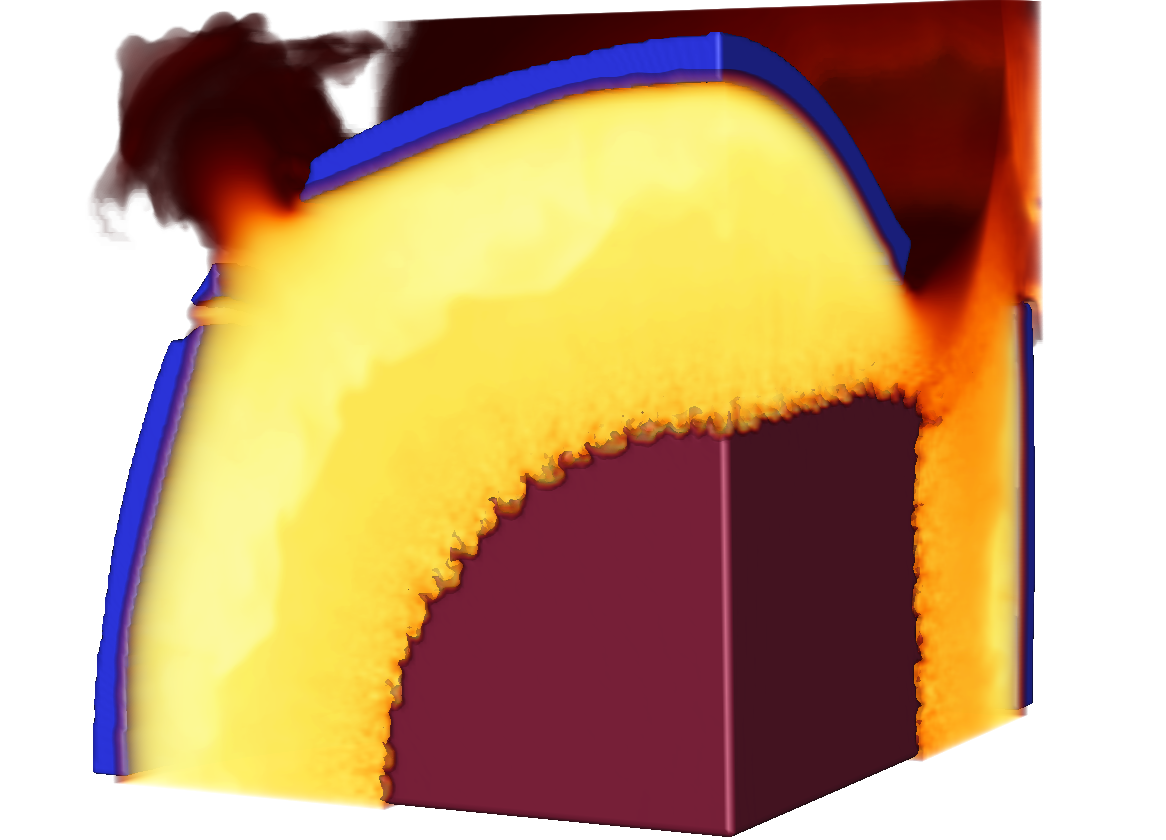
\includegraphics[width=\textwidth]{Figs/mpmice/NE_172_c.png}
   \caption{t=.312 $ms$}
   \label{figCookoff:e}
 \end{subfigure}
 \begin{subfigure}[b]{0.3\textwidth}
   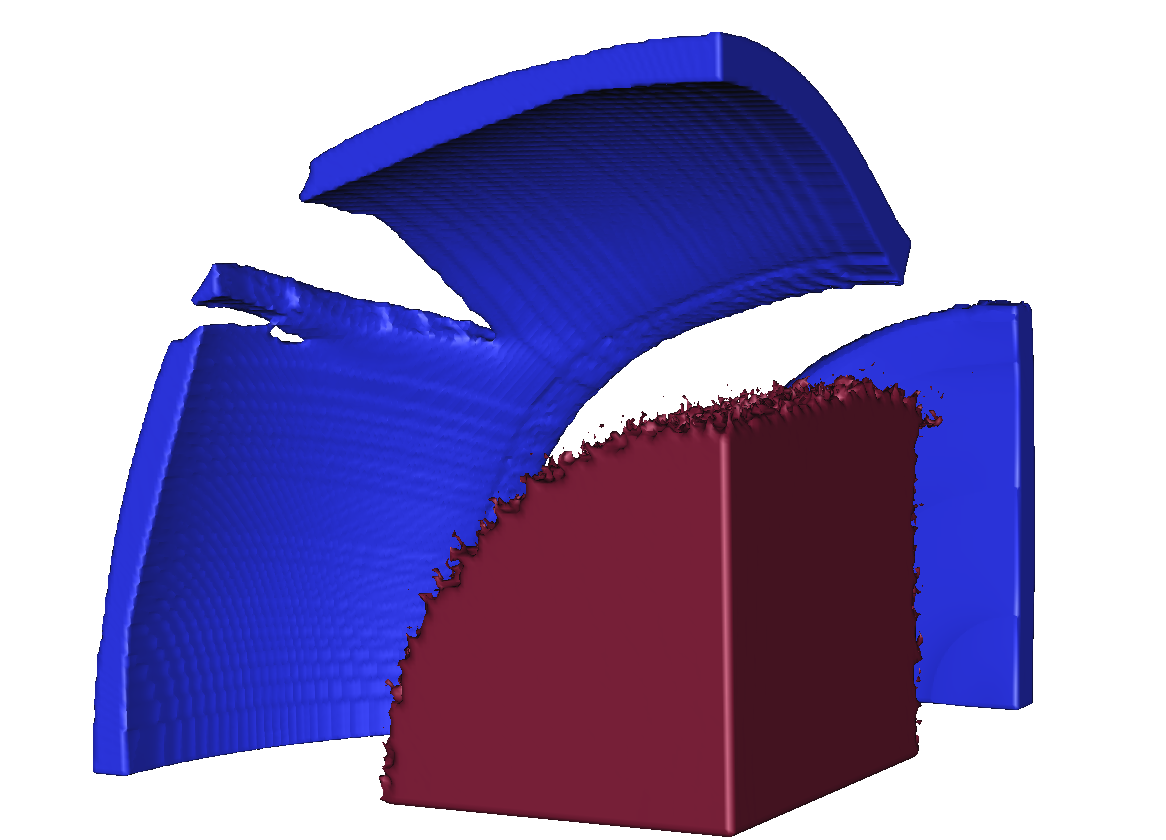
\includegraphics[width=\textwidth]{Figs/mpmice/NE_172_d.png}
   \caption{t=.312 $ms$}
   \label{figCookoff:f}
 \end{subfigure}
 \caption{Time series of a steel container (blue) filled with deflagrating 
          plastic bonded explosive(red).  A volume rendering of the mass 
          density of the products of reaction is also shown, except in the 
          final panel, where it is removed to more clearly show the regions 
          where the container has failed. }
 \label{figCookoff}
 \end{figure}

Since no surface tracking is required in this method, there is no
requirement to track the creation of the new surfaces that occur
due to material failure.  Gas is free to escape through the openings
simply because there is no longer anything in those computational
cells to prevent it once the gap is sufficiently wide.

